\section{Outside the lines}\label{sec:out}
\subsection{Commands}\label{sec:out:cmd}
\begin{command}{\tmlittlehalf\opt{\oarg{options}}}
  Give \tmlittlehalf. This is intended to be used in tempo text.
\end{command}
\begin{command}{\tmlittlehalfdot\opt{\oarg{options}}}
  Give \tmlittlehalfdot\ (|\tmlittlehalf| with a dot).
\end{command}
\begin{command}{\tmlittlequarter\opt{\oarg{options}}}
  Give \tmlittlequarter.
\end{command}
\begin{command}{\tmlittlequarterdot\opt{\oarg{options}}}
  Give \tmlittlequarterdot\ (|\tmlittlequarter| with a dot).
\end{command}
\begin{command}{\tmlittleeighth\opt{\oarg{options}}}
  Give \tmlittleeighth.
\end{command}
\begin{command}{\tmlittleeighthdot\opt{\oarg{options}}}
  Give \tmlittleeighthdot\ (|\tmlittleeighth| with a dot).
\end{command}
\begin{codeexample}[]
\begin{tmline}
\begin{tmstaff}{g}{}
  \path (1,1) node[right,font=\bfseries] {Slow, \tmlittleeighthdot[red]\ = 80};
\end{tmstaff}
\end{tmline}
\end{codeexample}
\subsection{Pics}\label{sec:out:pic}
To construct a music line, this package defines many different \tikzname\ pics. 
You can use them to define commands like in section \ref{sec:out:cmd}.
\subsubsection{Clefs}\label{sec:out:pic:clef}
\begin{pictype}{tm-g-clef}{}
  Draw a treble clef at normal size. When you use |\tmgclef| with |unscaled=false|, 
  the clef is scaled down to $0.8$ times its normal size.
\end{pictype}
\begin{pictype}{tm-c-clef}{}
  Draw an alto clef at normal size.
\end{pictype}
\begin{pictype}{tm-f-clef}{}
  Draw a bass clef at normal size.
\end{pictype}
\begin{codeexample}[]
\begin{tikzpicture}
  \begin{scope}
    \pic {tm-g-clef};
    \draw[red,ultra thin] (-.2,0) -- (.7,0) (0,1) -- (0,-1);
    \draw[blue,ultra thin] (-.2,-.4) -- (.7,-.4);
  \end{scope}
  \begin{scope}[xshift=1.5cm]
    \pic {tm-c-clef};
    \draw[red,ultra thin] (-.2,0) -- (.7,0) (0,1) -- (0,-1);
    \draw[blue,ultra thin] (-.2,-.4) -- (.7,-.4) (-.2,.4) -- (.7,.4);
  \end{scope}
  \begin{scope}[xshift=3cm]
    \pic {tm-f-clef};
    \draw[red,ultra thin] (-.2,0) -- (.7,0) (0,1) -- (0,-1);
    \draw[blue,ultra thin] (-.2,.2) -- (.7,.2) (-.2,.4) -- (.7,.4);
  \end{scope}
\end{tikzpicture}
\end{codeexample}
The bounding boxes of |tm-c-clef| and |tm-f-clef| is set to the same height of 
|tm-g-clef| so that the distances between staves of different clefs can be 
equally positioned.
\subsubsection{Note heads}\label{sec:out:pic:noteheads}
We have three main versions: the whole note, the half note and the quarter note. 
Each main version has three different sub-versions for three different values of 
|relative|.

Whole note pics:
\begin{pictype}{tm-whole-note-center}{}
  Draw a whole note.
\end{pictype}
\begin{pictype}{tm-whole-note-left}{}
  Draw a whole note.
\end{pictype}
\begin{pictype}{tm-whole-note-right}{}
  Draw a whole note.
\end{pictype}
The difference of the three pics:
\begin{codeexample}[]
\begin{tikzpicture}[scale=4,transform shape]
  \path (0,0)   pic       {tm-whole-note-center}
        (0,.1)  pic[red]  {tm-whole-note-right}
        (0,-.1) pic[blue] {tm-whole-note-left};
\end{tikzpicture}
\end{codeexample}

Half note pics:
\begin{pictype}{tm-half-note-head-center}{}
  Draw a half note head.
\end{pictype}
\begin{pictype}{tm-half-note-head-left}{}
  Draw a half note head.
\end{pictype}
\begin{pictype}{tm-half-note-head-right}{}
  Draw a half note head.
\end{pictype}
\begin{codeexample}[]
\begin{tikzpicture}[scale=4,transform shape]
\path (0,0)   pic       {tm-half-note-head-center}
      (0,.1)  pic[red]  {tm-half-note-head-right}
      (0,-.1) pic[blue] {tm-half-note-head-left};
\end{tikzpicture}
\end{codeexample}

Quarter note pics:
\begin{pictype}{tm-quarter-note-head-center}{}
  Draw a quarter note head.
\end{pictype}
\begin{pictype}{tm-quarter-note-head-left}{}
  Draw a quarter note head.
\end{pictype}
\begin{pictype}{tm-quarter-note-head-right}{}
  Draw a quarter note head.
\end{pictype}
\begin{codeexample}[]
\begin{tikzpicture}[scale=4,transform shape]
\path (0,0)   pic       {tm-quarter-note-head-center}
      (0,.1)  pic[red]  {tm-quarter-note-head-right}
      (0,-.1) pic[blue] {tm-quarter-note-head-left};
\end{tikzpicture}
\end{codeexample}
\subsubsection{Flags}\label{sec:out:pic:flags}
\begin{pictype}{tm-note-flag-up}{}
  Draw a flag for `up'-stems.
\end{pictype}
\begin{pictype}{tm-note-flag-down}{}
  Draw a flag for `down'-stems.
\end{pictype}
\begin{codeexample}[]
\begin{tikzpicture}[scale=2,transform shape]
  \draw[red] (0,-.5) -- (0,0);
  \pic at (0,0) {tm-note-flag-up};
  \draw[red] (1,0) -- (1,-.5);
  \pic at (1,-.5) {tm-note-flag-down};
\end{tikzpicture}
\end{codeexample}
\subsubsection{Rests}\label{sec:out:pic:rests}
Whole rest and half rest can be easily drawn with a simple rectangle, so there 
are no pics for them. Internally this is how they are drawn when |\tmwholerest| 
and |\tmhalfrest| are executed:
\begin{codeexample}[]
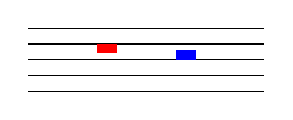
\begin{tikzpicture}
  \foreach \i in {-.4,-.2,0,.2,.4} \draw (0,\i) -- (3,\i);
  \fill[red] (.875,.08) rectangle ++ (.25,.12);
  \fill[blue] (1.875,0) rectangle ++ (.25,.12);
\end{tikzpicture}
\end{codeexample}
Other rests:
\begin{pictype}{tm-quarter-note-rest}{}
  Draw a quarter rest.
\end{pictype}
\begin{codeexample}[]
\begin{tikzpicture}
  \foreach \i in {-.4,-.2,0,.2,.4} \draw (0,\i) -- (2,\i);
  \pic[blue] at (1,0) {tm-quarter-note-rest};
\end{tikzpicture}
\end{codeexample}
For eighth rest and below, the pic name is |tm-|\meta{number}|-note-rest|, where 
\meta{number} is the number of `flags' in the rest notation. So |tm-1-note-rest| 
is the eighth rest, and so on. Currently \meta{number} must be either |1|,
|2|, |3| or |4|.
\begin{pictype}{tm-1-note-rest}{}
  Draw an eighth rest.
\end{pictype}
\begin{pictype}{tm-2-note-rest}{}
  Draw an sixteenth rest.
\end{pictype}
\begin{pictype}{tm-3-note-rest}{}
  Draw an thirty-second rest.
\end{pictype}
\begin{pictype}{tm-4-note-rest}{}
  Draw an sixty-fourth rest.
\end{pictype}
\begin{codeexample}[width=5.5cm]
\begin{tikzpicture}
  \foreach \i in {-.4,-.2,0,.2,.4} \draw (0,\i) -- (5,\i);
  \foreach \i in {1,2,3,4} \pic[blue] at (\i,0) {tm-\i-note-rest};
\end{tikzpicture}
\end{codeexample}

\subsubsection{Numbers}\label{sec:out:pic:numbers}
The pics draw musical numbers, taken from the music font \emph{Maestro}. Digit 
\meta{x} has a pic named |tm-number-|\meta{x}. By default, these pics are |4mm| 
high.
\foreach \i in {0,...,9} {%
\begin{pictype}{tm-number-\i}{}
  Draw number \i. \tikz\pic[scale=0.6]{tm-number-\i};
\end{pictype}%
}
Position in relative to the origin:
\begin{codeexample}[]
\begin{tikzpicture}
  \pic[scale=4] at (0,0) {tm-number-6};
  \draw[ultra thin,red] (0,1) -- (0,-1) (-1,0) -- (1,0);
\end{tikzpicture}
\end{codeexample}
\subsubsection{Other time signature notations}\label{sec:out:pic:time-signatures}
\begin{pictype}{tm-common-time}{}
  Draw common time notation. \tikz\pic[scale=0.6]{tm-common-time};
\end{pictype}
\begin{pictype}{tm-alla-breve-time}{}
  Draw alla breve time notation. \tikz\pic[scale=0.6]{tm-alla-breve-time};
\end{pictype}
\begin{codeexample}[]
\begin{tikzpicture}[scale=1.5,transform shape]
  \path (0,0) pic {tm-common-time} (1,0) pic {tm-alla-breve-time};
  \draw[ultra thin,red] (-.5,0) -- (1.5,0);
  \foreach \i in {0,1} \draw[ultra thin,red] (\i,.5) -- (\i,-.5);
\end{tikzpicture}
\end{codeexample}
\subsubsection{Accidentals}\label{sec:out:pic:accidentals}
\begin{pictype}{tm-sharp}{}
  Draw a sharp notation.
\end{pictype}
\begin{pictype}{tm-flat}{}
  Draw a flat notation.
\end{pictype}
\begin{pictype}{tm-natural}{}
  Draw a natural notation.
\end{pictype}
\begin{pictype}{tm-double-sharp}{}
  Draw a double sharp notation.
\end{pictype}
\begin{pictype}{tm-double-flat}{}
  Draw a double flat notation.
\end{pictype}
\begin{codeexample}[]
\begin{tikzpicture}[scale=1.5,transform shape]
  \foreach \i in {0,1,2,3,4} \draw[ultra thin,red] (\i,-.5) -- (\i,.5);
  \draw[ultra thin,red] (-.5,0) -- (4.5,0);
  \path (0,0) pic {tm-sharp} (1,0) pic {tm-flat} (2,0) pic {tm-natural}
    (3,0) pic {tm-double-sharp} (4,0) pic {tm-double-flat};
\end{tikzpicture}
\end{codeexample}
\subsubsection{Articulations}\label{sec:out:pic:articulations}
Only fermata notations are drawn using pics. Other articulations are all drawn 
using normal \tikzname\ commands. This is how those articulations are drawn 
internally:
\begin{codeexample}[]
\begin{tikzpicture}[scale=1.5,transform shape]
  \draw[line width=.1pt,red] (-.5,0) -- (4.5,0);
  \foreach \i in {0,1,2,3,4} \draw[line width=.1pt,red] (\i,.5) -- (\i,-.5);
  \fill[shift={(0,0)}] (0,0) circle (.4mm);%staccato
  \draw[shift={(1,0)}] (-.15,0) -- (.15,0);%tenuto
  \draw[shift={(2,0)}] (-.18,.075) -- (.18,0) -- (-.18,-.075);%accent above
  \fill[shift={(3,0)},rounded corners=.5pt]
    (0,.1) -- (-.04,-.075) to[out=-90,in=-90,looseness=2] (.04,-.075) -- cycle;%staccatissimo
  \draw[shift={(4,0)},fill]
    (-.1,-.1) -- (0,.1) -- (.1,-.1) -- (.033333,-.1) -- (-.033333,.0333333);%marcato
\end{tikzpicture}
\end{codeexample}
\begin{pictype}{tm-fermata-above}{}
  Draw a `fermata above' notation.
\end{pictype}
\begin{pictype}{tm-fermata-below}{}
  Draw a `fermata below' notation.
\end{pictype}
\begin{codeexample}[]
\begin{tikzpicture}
  \draw[line width=.1pt,red] (-.5,0) -- (1.5,0) (0,-.5) -- (0,.5) (1,-.5) -- (1,.5);
  \path (0,0) pic {tm-fermata-above} (1,0) pic {tm-fermata-below};
\end{tikzpicture}
\end{codeexample}
\subsubsection{Ornaments}\label{sec:out:pic:ornaments}
\begin{pictype}{tm-trill}{}
  Draw a trill.
\end{pictype}
\begin{pictype}{tm-turn}{}
  Draw a turn.
\end{pictype}
\begin{pictype}{tm-mordent}{}
  Draw a mordent.
\end{pictype}
\begin{codeexample}[width=5cm]
\begin{tikzpicture}[scale=1.5,transform shape]
  \draw[line width=.1pt,red] (-.5,0) -- (2.5,0);
  \foreach \i in {0,1,2} \draw[line width=.1pt,red] (\i,.5) -- (\i,-.5);
  \path (0,0) pic {tm-trill} (1,0) pic {tm-turn} (2,0) pic {tm-mordent};
\end{tikzpicture}
\end{codeexample}
That |tm-mordent| is the `upper' mordent. To have the `lower' version, this is 
how the package is drawing internally:
\begin{codeexample}[]
\begin{tikzpicture}[scale=2,transform shape]
  \draw[line width=.1pt,red] (-.5,0) -- (.5,0) (0,-.5) -- (0,.5);
  \path (0,0) pic {tm-mordent};
  \draw[line width=1pt] (0,-.15) -- (0,.15);
\end{tikzpicture}
\end{codeexample}
\subsubsection{Breath marks}\label{sec:out:pic:breath}
\begin{pictype}{tm-breath-mark}{}
  Draw a breath mark.
\end{pictype}
\begin{codeexample}[]
\begin{tikzpicture}[scale=2,transform shape]
  \draw[ultra thin,red] (-.5,0) -- (.5,0) (0,-.5) -- (0,.5);
  \pic at (0,0) {tm-breath-mark};
\end{tikzpicture}
\end{codeexample}
The caesura is not drawn using a pic. This is how it is drawn:
\begin{codeexample}[]

\begin{tikzpicture}[scale=2,transform shape]
  \foreach \i in {-.4,-.2,0,.2,.4} \draw (-.5,\i) -- (.5,\i);
  \fill[purple]
    (-.3,.2) -- (-.2,.2) -- (.1,.6) -- (0,.6) -- cycle
    (-.1,.2) -- (0,.2) -- (.3,.6) -- (.2,.6) -- cycle;
\end{tikzpicture}
\end{codeexample}
\subsubsection{Lines-related notations}\label{sec:out:pic:line}
Currently the following pics are defined:
\begin{pictype}{tm-8va}{}
  Draw a 8va notation.
\end{pictype}
\begin{pictype}{tm-8vb}{}
  Draw a 8vb notation.
\end{pictype}
\begin{pictype}{tm-15ma}{}
  Draw a 15ma notation.
\end{pictype}
\begin{pictype}{tm-15mb}{}
  Draw a 15mb notation.
\end{pictype}
\begin{codeexample}[width=4.5cm]
\foreach \i in {8va,8vb,15ma,15mb} {\tikz\pic{tm-\i};\quad}
\end{codeexample}
\begin{pictype}{tm-ped}{}
  Draw the stylised \emph{ped} used in pedal lines.
\end{pictype}
\begin{pictype}{tm-ped-star}{}
  Draw the star used in pedal lines.
\end{pictype}
\begin{codeexample}[]
\begin{tikzpicture}
  \draw (0,0) pic {tm-ped} -- (3,0) pic {tm-ped-star};
\end{tikzpicture}
\end{codeexample}
\subsubsection{Dynamics}\label{sec:out:pic:dynamics}
\foreach \i in {mf,f,ff,fff,mp,p,pp,ppp,fp} {%
\begin{pictype}{tm-dynamics-\i}{}
  Draw dynamics notation \texttt{\i}.
\end{pictype}%
}
\begin{codeexample}[]
\foreach \i in {mf,f,ff,fff,mp,p,pp,ppp,fp} {\tikz\pic{tm-dynamics-\i};\quad}
\end{codeexample}
